\documentclass[12pt,fleqn]{beamer}


\xdefinecolor{lavendar}{rgb}{0.8,0.6,1}
\xdefinecolor{olive}{cmyk}{0.64,0,0.95,0.4}
%\xdefinecolor{olive}{cmyk}{1,0,0,0}
\xdefinecolor{mag}{cmyk}{0.1,1,0,0.2}
\xdefinecolor{lblue}{rgb}{0,0,1.5}
\xdefinecolor{lred}{rgb}{1,0,0}
\xdefinecolor{mine}{cmyk}{1,0,0.2,0}
\xdefinecolor{bluel}{cmyk}{0.1,0,0.9,0.4}

\usepackage{amsmath,amssymb,dsfont,mathrsfs}
\usepackage{tikz,pgflibraryplotmarks}
\usepackage{multimedia}
\usepackage{wasysym}
\usepackage{rotating}
\usepackage{algorithm,algorithmic}
\usepackage{graphicx} % more modern
\usepackage{subfigure}
\usepackage{booktabs}

\usepackage{pgfplots}
\usepackage{verbatim}

\usepackage{setspace}
\newlength\iwidth
\newlength\iheight

\newcommand\makebeamertitle{\frame{\maketitle}}%
\graphicspath{{./images/}}
\setbeamertemplate{navigation symbols}{}
\addtobeamertemplate{navigation symbols}{}{%
    \usebeamerfont{footline}%
    \usebeamercolor[fg]{footline}%
	\insertshorttitle
    \;--
    \insertframenumber
}

\newcommand{\sectionstart}{
	\only<beamer>{
 	\begin{frame}% (fold)
 		\begin{centering}\Huge \insertsection \par\end{centering}
 	\end{frame}% frame the_application (end)
	}
 }


% make bibliography entries smaller
\usepackage{natbib}
\setbeamertemplate{bibliography item}{[\theenumiv]}
\renewcommand\bibfont{\scriptsize}
\setbeamertemplate{frametitle continuation}[from second]
\newcommand{\tcr}{\textcolor{red}}
\newcommand{\tcrd}{\textcolor{red}}
\newcommand{\tcb}{\textcolor{bluel}}
\newcommand{\tcm}{\textcolor{mag}}
\newcommand{\tcg}{\textcolor{olive}}

\newcommand{\R}{\mathbb{R}}
\newcommand{\C}{\mathbb{C}}

% bold lower-case for vectors
\newcommand{\bfa}{{\bf a}}
\newcommand{\bfb}{{\bf b}}
\newcommand{\bfc}{{\bf c}}
\newcommand{\bfs}{{\bf s}}
\newcommand{\bfm}{{\bf m}}
\newcommand{\bfd}{{\bf d}}
\newcommand{\bfe}{{\bf e}}
\newcommand{\bfu}{{\bf u}}
\newcommand{\bfy}{{\bf y}}
\newcommand{\bfx}{{\bf x}}
\newcommand{\bfh}{{\bf h}}
\newcommand{\bfw}{{\bf w}}
\newcommand{\bfv}{{\bf v}}
\newcommand{\bfr}{{\bf r}}
\newcommand{\bfz}{{\bf z}}
\newcommand{\bfp}{{\bf p}}


% bold upper-case for linear operators
\newcommand{\bfA}{{\bf A}}
\newcommand{\bfB}{{\bf B}}
\newcommand{\bfZ}{{\bf Z}}
\newcommand{\bfM}{{\bf M}}
\newcommand{\bfC}{{\bf C}}
\newcommand{\bfD}{{\bf D}}
\newcommand{\bfQ}{{\bf Q}}
\newcommand{\bfJ}{{\bf J}}
\newcommand{\bfG}{{\bf G}}
\newcommand{\bfI}{{\bf I}}
\newcommand{\bfP}{{\bf P}}
\newcommand{\bfK}{{\bf K}}
\newcommand{\bfY}{{\bf Y}}
\newcommand{\bfW}{{\bf W}}
\newcommand{\bfR}{{\bf R}}
\newcommand{\bfL}{{\bf L}}
\newcommand{\bfF}{{\bf F}}
\newcommand{\bfT}{{\bf T}}
\newcommand{\bfS}{{\bf S}}
\newcommand{\bfX}{{\bf X}}
\newcommand{\bfU}{{\bf U}}
\newcommand{\bfV}{{\bf V}}
\newcommand{\bfH}{{\bf H}}


\newcommand{\calF}{\mathcal{F}}



\newcommand{\hf}{{\frac 12}}
\newcommand{\bftheta}{{\boldsymbol \theta}}
\newcommand{\bfxi}{{\boldsymbol \xi}}

\newcommand{\bfLambda}{{\boldsymbol \Lambda}}
\newcommand{\bfSigma}{{\boldsymbol \Sigma}}
\newcommand{\bfepsilon}{{\boldsymbol \epsilon}}

\newcommand{\E}{\vec E}
\newcommand{\B}{\vec B}

\newcommand{\vu}{  {\vec {\bf u}}}

\newcommand{\grad}{  {\vec {\bf \nabla}}}

\newcommand{\lfrownie}{\textcolor{red}{\large{\frownie}}}
\newcommand{\lsmiley}{\textcolor{green}{\large{\smiley}}}

\newcommand{\curl}{\ensuremath{\nabla\times\,}}
\renewcommand{\div}{\nabla\cdot\,}
\newcommand{\divh}{\nabla_h\cdot\,}
\renewcommand{\grad}{\ensuremath{\nabla}}

\DeclareMathOperator*{\argmin}{arg\,min}
\date{}


\title{Deep Neural Networks}
\subtitle{Numerical Methods for Deep Learning}

\begin{document}

\makebeamertitle

\section{Motivation} % (fold)
\label{sec:motivation}
\begin{frame}[fragile]\frametitle{Why Deep Networks?}

\begin{itemize}
\item Universal approximation theorem of NN suggests that we can approximate {\bf any} function by
two layers.
\item But - The width of the layer can be very large ${\cal O}(n\cdot n_f)$
\item
Deeper architectures can lead to more efficient descriptions of the problem.

(No real proof but lots of practical experience)
\end{itemize}

\end{frame}





\begin{frame}
	\frametitle{Learning Objective: Deep Neural Networks}
	
	In this module we introduce multilayer deep neural networks.
	
	\bigskip
	
	Learning tasks:
	\begin{itemize}
		\item regression
		\item classification
	\end{itemize}
	
	\bigskip
	
	Numerical methods:
	\begin{itemize}
		\item non-convex optimization
		\item probability theory (for initialization)
	\end{itemize}
\end{frame}


\begin{frame}[fragile]\frametitle{Deep Neural Networks}


Until recently, the standard architecture was
\begin{eqnarray*}
\bfY_1 &=& \sigma(\bfK_0\bfY_0 + \bfb_0) \\
\vdots & =&  \vdots \\
 \bfY_N &=& \sigma(\bfK_{N-1}  \bfY_{N-1}+ \bfb_{N-1})
 \end{eqnarray*}

\bigskip
\pause

And use $\bfY_N$ to classify. This leads to the optimization problem
$$ 
\min_{\bfK_{0,\ldots,N-1},\bfb_{0,\ldots,N-1},\bfW} \ \ E\left(\bfW \bfY_N(\bfK_1,\ldots,\bfK_{N-1},\bfb_1,\ldots, \bfb_{N-1}) , \bfC^{\rm obs} \right)
 $$

\pause

\bigskip

How deep is deep? For now, let's say $N>1$.
\end{frame}

\begin{frame}
	\frametitle{Example: Hand-written digit recognition~\cite{LeCun1990}}
	
	\begin{description}
		\item[layer 1:] 
			\begin{itemize}
				\item input features: images of size $28 \times 28$
				\item $\bfK_1$: four $5\times5$ convolution stencils.
				\item $\bfb_1 \in \R^4$ are biases
				\item $\sigma = \tanh$
				\item output features: four images of size $24\times 24$				
			\end{itemize}
		\item[layer 2:] average pooling (no trainable weights)
		\item[layer 3:] 
			\begin{itemize}
				\item input features: four images of size $12 \times 12$
				\item $\bfK_2$: 48 $5\times5$ convolution stencils.
				\item $\bfb_2 \in \R^4$ are biases
				\item $\sigma = \tanh$
				\item output features: four images of size $12\times 12$				
			\end{itemize}
		\item[layer 4:] average pooling (no trainable weights)
	\end{description}
	
	\bigskip
	\pause
	
	Very effective for MNIST, but today's architectures have become more sophisticated.
	
\end{frame}

\begin{frame}\frametitle{Example: The Alexnet~\cite{KrizhevskySutskeverHinton2012} for Image Classification}

\begin{columns}
	\column{.6\textwidth}
	\begin{itemize}
		\item Complex architectures 
		\item trained on multiple GPUs
		\item $\approx $ 60 million weights
	\end{itemize}	
	\column{.4\textwidth}
\begin{center}
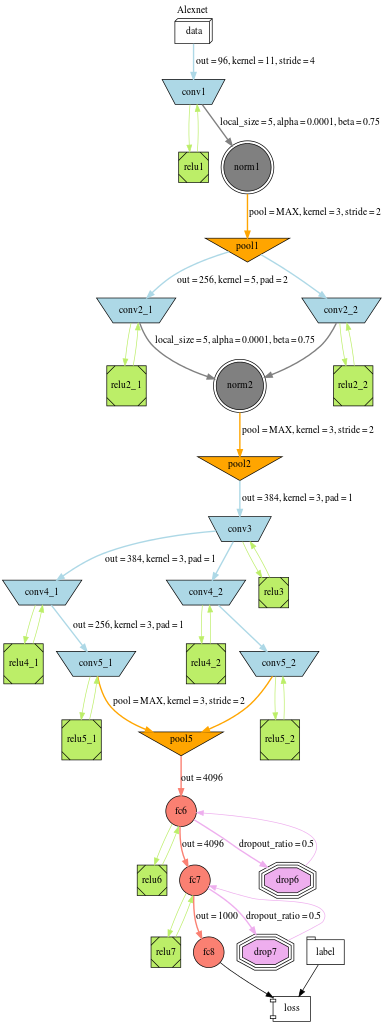
\includegraphics[width=2.9cm]{Alexnet-wikimedia}
\end{center}
\end{columns}
\end{frame}

\begin{frame}
	\frametitle{Key issues: Non-Convexity and Initialization}
	
	Optimization problems in learning are generally non-convex.
	
	\begin{itemize}
		\item training relies on stochastic gradient methods~\cite{bottou2016optimization}
		\item initialization is key~\cite{GlorotBengio2010}
	\end{itemize}
	

	\bigskip
	
	Initialization is particularly important.  Simple example:
	Let $\bfy\in\R^{100} \sim \mathcal{N}(0,\bfI)$	Compare
	\begin{equation*}
		\|\bfK_3 \bfK_2 \bfK_1 \bfy \|^2 \quad \text{ to } \quad\|\bfy \|
	\end{equation*}
	for different choices of $\bfK_1,\bfK_2,\bfK_3 \in \R^{100\times 100}$. Sample entries independently, e.g., from standard normal,  uniform in $[-0.5,0.5]$, uniform in $[-0.05,0.05]$. 	See more details in~\cite{GlorotBengio2010}. 
	
\end{frame}


\section{Summary} % (fold)
\label{sec:numerical_optimization}
\begin{frame}[fragile]\frametitle{$\Sigma$: Deep Neural Networks}

Idea: Concatenate many single layers and solve
$$ 
\min_{\bfK_{0,\ldots,N-1},\bfb_{0,\ldots,N-1},\bfW} \ \ E\left(\bfW \bfY_N(\bfK_1,\ldots,\bfK_{N-1},\bfb_1,\ldots, \bfb_{N-1}) , \bfC^{\rm obs} \right)
 $$


Discussion:
\begin{itemize}
	\item empirically shown for some examples to generalize better and be more efficient than wide architectures 
	\item 
Challenge 1: computational costs (architecture have millions or billions of parameters)
	\item Challenge 2: design architecture that is easy to train and generalizes well
	\item Challenge 3: learning leads to very non-convex optimization problems $\leadsto$ initialization is key. Leads to exploding/vanishing gradient phenomena.
\end{itemize}
\end{frame}



\begin{frame}[allowframebreaks]
	\frametitle{References}
\bibliographystyle{abbrv}
\bibliography{NumDNN}

\end{frame}

\end{document}
